\chapter{Autoregressive neural networks (ARNN)}
\label{sec:arnn}

\section{Dense and convolutional ARNN}

\cite{wu2019solving}

\cite{nicoli2020asymptotically}

\cite{ciarella2023machine}

\begin{figure}[htb]
\centering
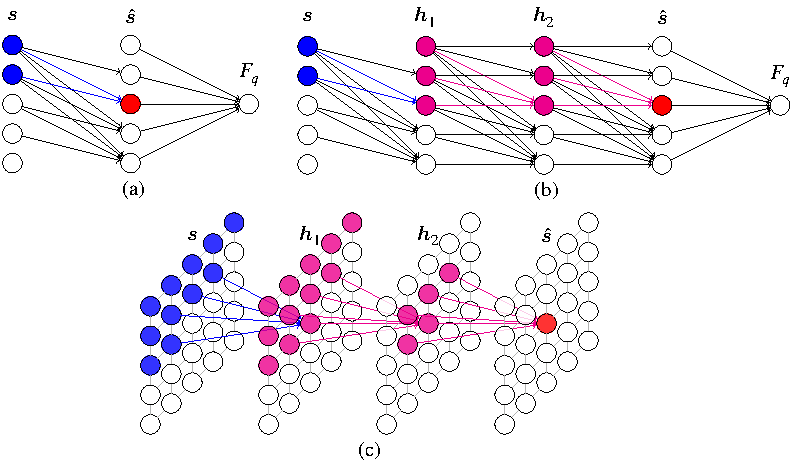
\includegraphics[width=0.9\linewidth]{ch3/arnn_arch.pdf}
\caption[Architectures of autoregressive neural networks for variational inference]{
Architectures of autoregressive neural networks (ARNN) for variational inference.
The spin configuration $\vs$ is the input to the network, $\hat{\vs}$ is the output of the network, and $h$ denotes hidden layer. The loss function $F_q$ is given by \cref{eq:fq}. The colored sites denote the receptive field of a site in $\hat{\vs}$.
(a) The network has only one layer, which is densely connected, while the autoregressive property hold.
(b) The network has a hidden layer.
(c) The network has masked convolution layers on 2D lattice. Only connections in a convolution kernel are shown for clarity.
}
\label{fig:arnn-arch}
\end{figure}

\subsection{Numerical results}

\begin{figure}[htb]
\centering
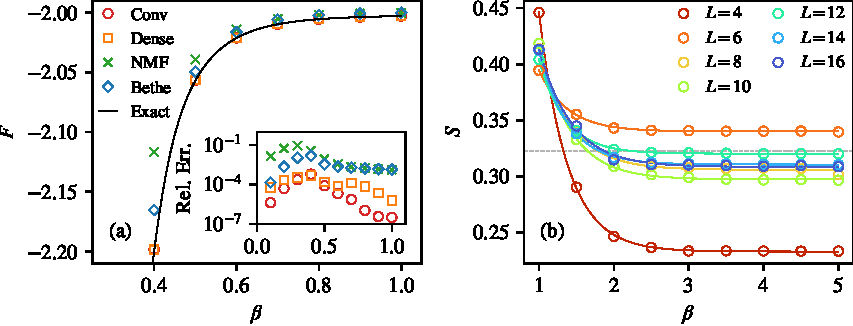
\includegraphics[width=\linewidth]{ch3/arnn_ising.pdf}
\caption[ARNN results of Ising model on square and triangular lattices]{
(a) Free energy per site of the ferromagnetic Ising model on the $16 \times 16$ square lattice with periodic boundary condition.
(b) Entropy per site of the antiferromagnetic Ising model on triangular lattices of various sizes $L$ with periodic boundary condition.
The exact result (dashed line) at $T = 0$ and $L \to \infty$ is $S / N = 0.323066$~\cite{TODO}. The curves for $L = 8, 14, 16$ are almost overlapped.
}
\label{fig:arnn-ising}
\end{figure}

\begin{figure}[htb]
\centering
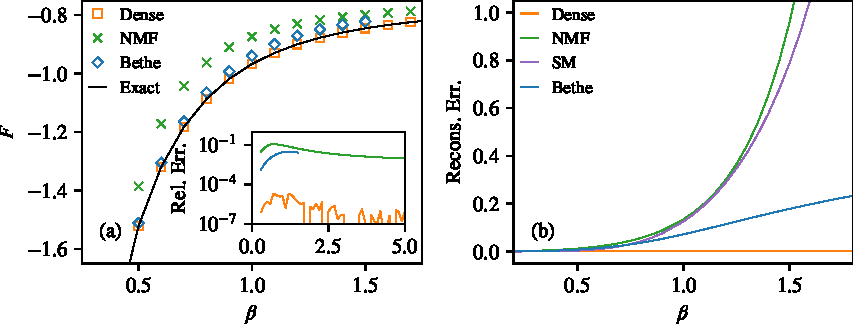
\includegraphics[width=\linewidth]{ch3/arnn_sk.pdf}
\caption[ARNN results of Sherrington--Kirkpatrick model]{
(a) Free energy per site and (b) entropy per site of the Sherrington--Kirkpatrick (SK) model with $N = 20$ spins.
}
\label{fig:arnn-sk}
\end{figure}

\begin{figure}[htb]
\centering
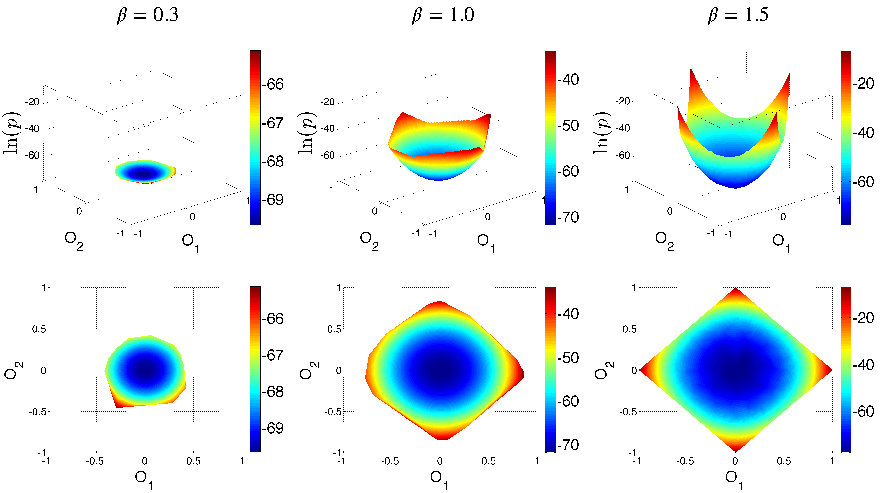
\includegraphics[width=\linewidth]{ch3/arnn_hop.pdf}
\caption[ARNN results of Hopfield model]{
Log probability of sampled configurations of ARNN learned for a Hopfield model with $N = 100$ spins, and $P = 2$ orthogonal patterns, on the two-dimensional spaces spanned by two patterns. In the figures, the $x$- and the $y$-axes represent inner product (overlap) between each sampled configuration and the first and the second stored patterns respectively. Our network uses single layer and only $N (N - 1) / 2$ parameters. The top figures are 3D view of the meshed log probability surface, while the bottom figures are the 2D view from top. From left to right, $\beta$ values are $0.3$, $1.0$, and $1.5$ respectively.
\todo{Reformat this plot if we have time}
}
\label{fig:arnn-hop}
\end{figure}

\section{Sparse two-body ARNN}

\cite{biazzo2024sparse}

\subsection{Numerical results}

\section{ARNN in MCMC importance sampling}

\subsection{Neural cluster updates}
\label{sec:ncus}

\cite{wu2021unbiased}

\subsection{Numerical results}
